Begge databasetyper besidder styrker og svagheder, men der er nogle klare fordele ved NoSQL. NoSQL databaser bygger ofte på en scale-out strategi, som gør det lettere og billigere af skalere op til store mængder data end SQL og dets scale-up tilgang.

Scale-up strategien går ud på, at forbedr computeren(serveren) med stærkere hardware, så det kan lagre mere data og gør performance hurtigere. Strategien er i praksis mere begrænset end hvad den er teoretisk. Teoretisk vil man kunne opgradere computeren med hurtigere processorer, mere RAM og mere lagerplads, men databasens bottleneck bevæger sig fra at være langsomt hardware til netværksforbindelse. Scale-up strategien er baseret på en enkelt computer frem for at sprede dataen ud over flere lokationer.

Scale-out strategien som NoSQL bruger er hvor der laves replicas af dataen og distribuerer ud på flere maskiner, ikke nødvendigvis lige så stærke og dyre maskiner. Denne strategi er billigere end Scale-up men det kan komme med nogle ulemper når det angår skrivning af ny data. Ulempen forekommer dog kun hvis der er en enorm mængde af nye skrivninger på samme tid. Eftersom det er replicas af dataen de fleste maskiner besidder, skal disse holdes ajour, så dataen ikke forældes. Hvori problemet opstår.

For at illustrere de to forskellige skalerings metoder, kan man forestille sig det som en byggeplan. Hvis man scaler op så er det som at sætte flere etager på en bygning, på et tidspunkt kan man bare ikke sætte flere etager ovenpå. Med scale out strategien tilføjer man bare flere bygninger, se illustration på figur \ref{fig::scaling}. 

\begin{figure}
    \centering
    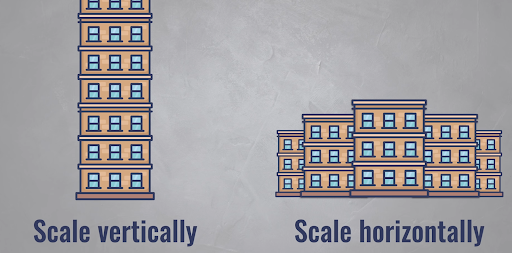
\includegraphics[scale=0.5]{scaling.png}
    \caption{Illustrering af scaling med database.}
    \label{fig::scaling}
\end{figure}

NoSQL er baseret på key-value par, hvor at hver række har en primær nøgle som har en korresponderende værdi. Værdien behøves ikke bare f.eks. være et navn på et produkt, men kan være en hel JSON streng, og siden at NoSQL er skemaløst, behøver alle værdierne ikke følge samme struktur. Som nævnt tidligere er NoSQL databaser ‘eventually consistent’, som vil sige at hvis et element i databasen er blevet tilføjet eller opdateret og man derefter prøver at læse elementet, er det ikke sikkert at det findes eller er opdateret. Hvis man kun har et lille system eller hjemmeside benytter man sig højst sandsynlig kun af en enkelt partition, og så er det ikke et problem at dataen er eventually consistent. Selv i praksis så bliver data kopieret mellem mirrors over millisekunder, og det er ikke det helt store problem når vi befinder os i den lave ende af write requests mod databasen, på den anden side hvis man har et system som får flere tusinde write requests i sekunder som hele tiden skal kopieres, kan det blive et problem hvis en person henter data der i mellemtiden er blevet forældet. Ved alt som forklaret her har NoSQL mange styrker til at kunne håndtere store mængder at data, holde styr på dem og have flere forskellige strukturer af data. NoSQL er virkelig hurtig til at hente enkelte elementer ud fra f.eks. et index, men hvis man f.eks. gerne vil analysere data og gerne vil se alle produkter man har der koster mere end 100 kr. vil NoSQL være utrolig langsom til dette, hvor det slet ikke ville være et problem for SQL. 
